\documentclass[12pt, titlepage]{article}

\usepackage{booktabs}
\usepackage{graphicx}
\usepackage{tabularx}
\usepackage{hyperref}
\usepackage{tabto}
\usepackage{amsmath}
\hypersetup{
    colorlinks,
    citecolor=blue,
    filecolor=black,
    linkcolor=red,
    urlcolor=blue
}
\usepackage[round]{natbib}

%% Comments

\usepackage{color}

\newif\ifcomments\commentstrue %displays comments
%\newif\ifcomments\commentsfalse %so that comments do not display

\ifcomments
\newcommand{\authornote}[3]{\textcolor{#1}{[#3 ---#2]}}
\newcommand{\todo}[1]{\textcolor{red}{[TODO: #1]}}
\else
\newcommand{\authornote}[3]{}
\newcommand{\todo}[1]{}
\fi

\newcommand{\wss}[1]{\authornote{blue}{SS}{#1}} 
\newcommand{\plt}[1]{\authornote{magenta}{TPLT}{#1}} %For explanation of the template
\newcommand{\an}[1]{\authornote{cyan}{Author}{#1}}

%% Common Parts

\newcommand{\progname}{ProgName} % PUT YOUR PROGRAM NAME HERE
\newcommand{\authname}{Team \#, Team Name
\\ Student 1 name
\\ Student 2 name
\\ Student 3 name
\\ Student 4 name} % AUTHOR NAMES                  

\usepackage{hyperref}
    \hypersetup{colorlinks=true, linkcolor=blue, citecolor=blue, filecolor=blue,
                urlcolor=blue, unicode=false}
    \urlstyle{same}
                                


\begin{document}

\title{Simulating Turbulent Flow with Synthetic Eddy: System Verification and Validation Plan for \progname{}}
\author{\authname}
\date{\today}
	
\maketitle

\pagenumbering{roman}

\section*{Revision History}

\begin{tabularx}{\textwidth}{p{3cm}p{2cm}X}
\toprule {\bf Date} & {\bf Version} & {\bf Notes}\\
\midrule
2024-02-19 & 1.0 & Initial Plan After SRS\\
\bottomrule
\end{tabularx}

% ~\\
% \wss{The intention of the VnV plan is to increase confidence in the software.
% However, this does not mean listing every verification and validation technique
% that has ever been devised.  The VnV plan should also be a \textbf{feasible}
% plan. Execution of the plan should be possible with the time and team available.
% If the full plan cannot be completed during the time available, it can either be
% modified to ``fake it'', or a better solution is to add a section describing
% what work has been completed and what work is still planned for the future.}

% \wss{The VnV plan is typically started after the requirements stage, but before
% the design stage.  This means that the sections related to unit testing cannot
% initially be completed.  The sections will be filled in after the design stage
% is complete.  the final version of the VnV plan should have all sections filled
% in.}

\newpage

\tableofcontents

\listoftables
% \wss{Remove this section if it isn't needed}

\listoffigures
% \wss{Remove this section if it isn't needed}

\newpage

\section{Symbols, Abbreviations, and Acronyms}

Please refer to the Software Requirements Specification (SRS) \citet{SRS} of this project. Section 1 contains Symbols, Abbreviations, and Acronyms. If you are not familiar with fluids and CFD, Section 4.1.1 of the SRS contains a list of Terminology and Definitions.\\
~\newline
The following symbols and operators are used in this document:\\
\renewcommand{\arraystretch}{1.2}
\begin{tabular}{l l} 
  \toprule		
  \textbf{symbol} & \textbf{description}\\
  \midrule 
  tol & Tolerance, a small value used when testing differences, see \ref{secSymParams}\\
  std() & Standard deviation of multiple values.\\
  div() & Divergence of a velocity field.\\
  \bottomrule
\end{tabular}\\

% \wss{symbols, abbreviations, or acronyms --- you can simply reference the SRS
%   \citep{SRS} tables, if appropriate}

% \wss{Remove this section if it isn't needed}

\newpage

\pagenumbering{arabic}

This document lays the plan for the verification and validation of the software \progname{}. It provides an overview of what the tests aim to achieve, and then details the plan for each test. It also serves as a communication aid between the software development team and the domain experts on the theoretical side, so that it can be ensured that the correct aspect of the software is being tested with valid expectations.
% ... \wss{provide an introductory blurb and roadmap of the
  % Verification and Validation plan}

\section{General Information}

\subsection{Summary}

The software being tested is a program that generates approximated turbulent flow field with synthetic eddies. It is intended to provided initial and boundary conditions (IC and BC) to CFD solvers for turbulent flow simulations, which would cut down simulation time and save computational resources. An illustration of the flow field that the software is intended to generate is shown in Figure \ref{Fig_PhysicalSystem}.

\begin{figure}[h!]
  \begin{center}
   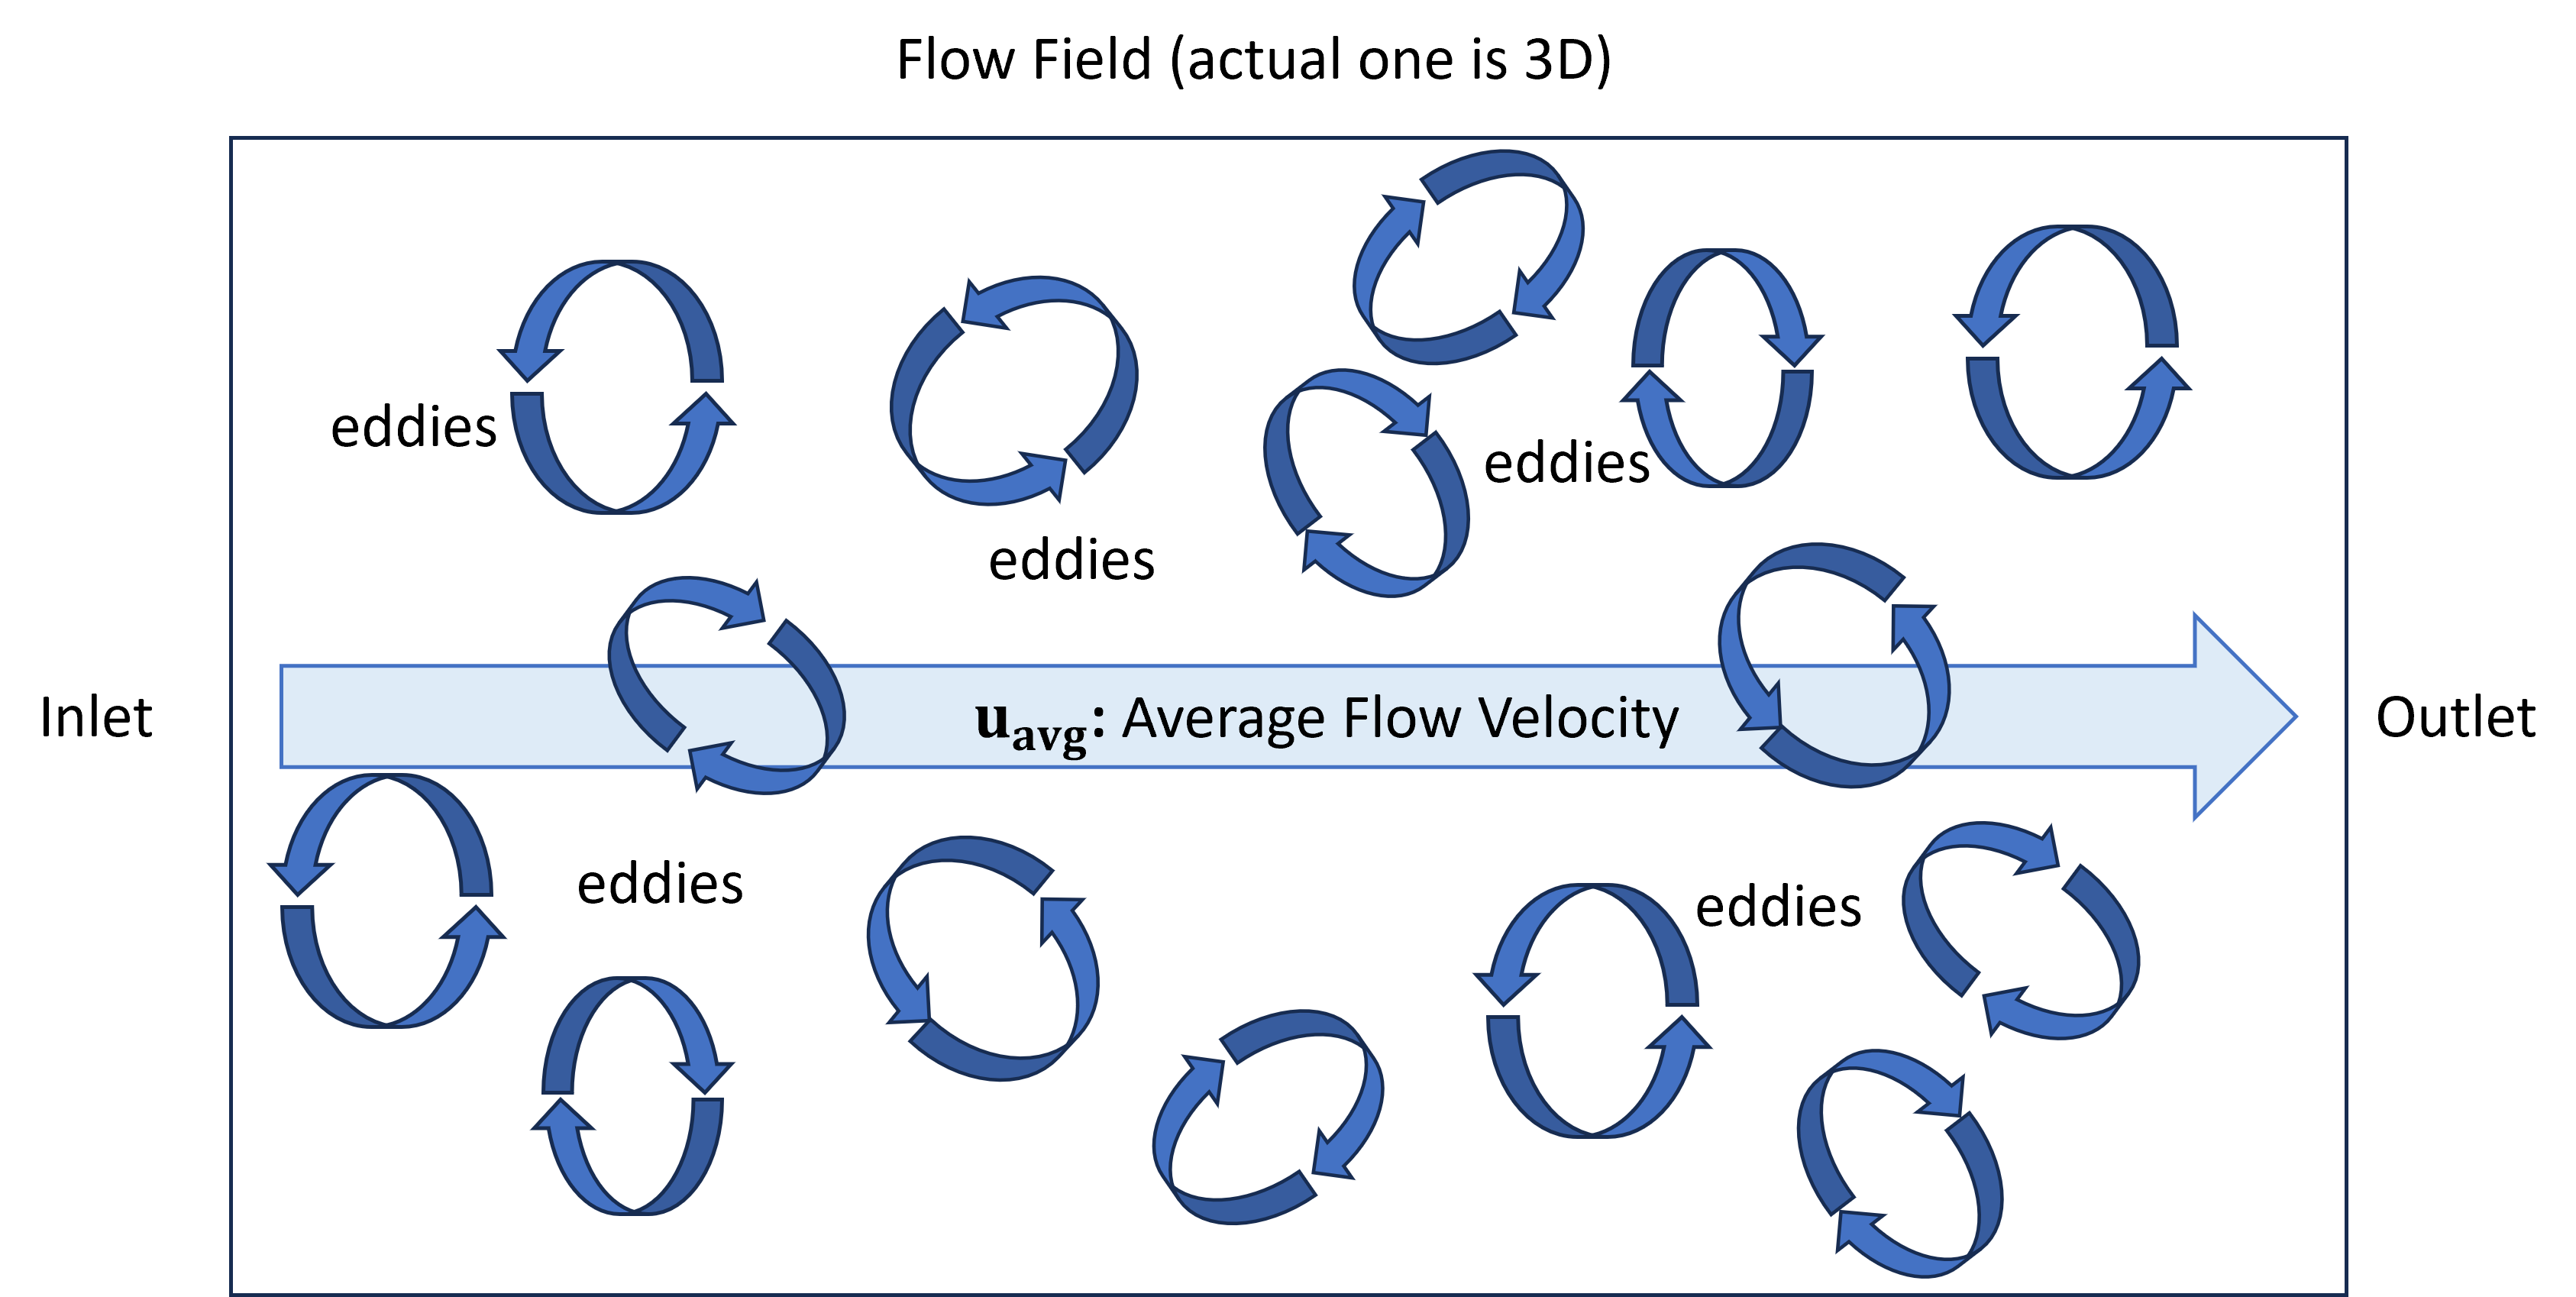
\includegraphics[width=0.8\textwidth]{PS.png}
  \caption{System Context}
  \label{Fig_PhysicalSystem} 
  \end{center}
\end{figure}


% \wss{Say what software is being tested.  Give its name and a brief overview of
%   its general functions.}

\subsection{Objectives}

The most crucial objective here is to build confidence that this software can correctly generate turbulent flow fields according to the synthetic eddy method proposed by \cite{PolettoEtAl2013}. As no suitable pseudo-oracle exists to allow for direct comparison of the results, the focus is to test for characteristics that a flow field generated with such method should exhibit. In the future with more theoretical background given, this will expand to making sure the generated flow fields are physically realistic in terms of turbulent properties. 

Another objective is to demonstrate the this software can interface with CFD solvers and provide in order to IC and BC for turbulent flow simulations (future development).

Furthermore, maintainability, namely the ability for user to easily modify the software to fit their specific needs should also be demonstrated.

% \wss{State what is intended to be accomplished.  The objective will be around
%   the qualities that are most important for your project.  You might have
%   something like: ``build confidence in the software correctness,''
%   ``demonstrate adequate usability.'' etc.  You won't list all of the qualities,
%   just those that are most important.}

% \wss{You should also list the objectives that are out of scope.  You don't have 
% the resources to do everything, so what will you be leaving out.  For instance, 
% if you are not going to verify the quality of usability, state this.  It is also 
% worthwhile to justify why the objectives are left out.}

% \wss{The objectives are important because they highlight that you are aware of 
% limitations in your resources for verification and validation.  You can't do everything, 
% so what are you going to prioritize?  As an example, if your system depends on an 
% external library, you can explicitly state that you will assume that external library 
% has already been verified by its implementation team.}

\subsection{Relevant Documentation}

\begin{itemize}
  \item Software Requirements Specification (SRS) \citet{SRS} is the most important guideline for this VnV plan. It contains the requirements of the software, and the theoretical Modules of the synthetic eddy method. 
  \item Design Documents will be used to guide the unit testing and the design verification.
\end{itemize}

% \wss{Reference relevant documentation.  This will definitely include your SRS
%   and your other project documents (design documents, like MG, MIS, etc).  You
%   can include these even before they are written, since by the time the project
%   is done, they will be written.}

% \wss{Don't just list the other documents.  You should explain why they are relevant and 
% how they relate to your VnV efforts.}

\section{Plan}

This section lays out how the VnV will be carried out in aspect and by whom. It also includes the tools that will be used for the VnV.

% \wss{Introduce this section.   You can provide a roadmap of the sections to
%   come.}

\subsection{Verification and Validation Team}

\begin{itemize}
  \item Phil Du - Developer: Writing test scripts according to VnV and implementing automated tests with continuous integration (CI). Ensuring coding standards are respected with linters.
  \item Nikita Holyev - Theorist: Reviewing the VnV plan to ensure that the tests are relevant to the theoretical models.
  \item Cynthia Liu - Subject Matter Expert: Reviewing the VnV plan and design documents to make sure the SRS is met.
  \item Morteza Mirzaei - Secondary reviewer of the VnV plan.
  \item Dr. Spencer Smith - Supervisor.
  \item Several volunteers as subjects for usability (future) and maintainability testing.
\end{itemize}

% \wss{Your teammates.  Maybe your supervisor.
%   You should do more than list names.  You should say what each person's role is
%   for the project's verification.  A table is a good way to summarize this information.}

\subsection{SRS Verification Plan}

Most of the Functional Requirements in the SRS \citet{SRS}, namely R1-R4 are derived from the synthetic eddy method by \citet{PolettoEtAl2013}, and can be represented mathematically. Thus, they are covered by automated testing detailed in Section \ref{FuncTest}. R5, the interface with CFD software, need to be verified with manual testing by actually conducting CFD simulations with the generated IC and BC.

The Nonfunctional Requirements in the SRS, including Accuracy, Usability, Maintainability and Portability, will be verified by manual testing. All of these other than Maintainability involves running the software in conjecture with CFD solvers, and will be performed when the CFD integration is implemented in the future. Maintainability will be verified by persons other than the developer attempting to modify the software, and is detailed in Section \ref{NonfuncTest}.

The Functional and Nonfunctional Requirements in the SRS serve as a checklist.

% \wss{List any approaches you intend to use for SRS verification.  This may include
%   ad hoc feedback from reviewers, like your classmates, or you may plan for 
  % something more rigorous/systematic.}

% \wss{Maybe create an SRS checklist?}

\subsection{Design Verification Plan}

\textit{Pending design documents.}

\wss{Plans for design verification}

\wss{The review will include reviews by your classmates}

\wss{Create a checklists?}

\subsection{Verification and Validation Plan Verification Plan}

The VnV plan itself is verified by review. The developer and reviewers will ensure that all the requirements in the SRS are covered by the plan. The theorist will specifically review the flow field tests to ensure that they represent the theoretical characteristics of the synthetic eddy method.

% \wss{The verification and validation plan is an artifact that should also be
% verified.  Techniques for this include review and mutation testing.}

% \wss{The review will include reviews by your classmates}

% \wss{Create a checklists?}

\subsection{Implementation Verification Plan}

Successful implementation of the synthetic eddy method can be verified by automated tests detailed in Section \ref{FuncTest}.

% \wss{You should at least point to the tests listed in this document and the unit
%   testing plan.}

% \wss{In this section you would also give any details of any plans for static
%   verification of the implementation.  Potential techniques include code
%   walkthroughs, code inspection, static analyzers, etc.}

\subsection{Automated Testing and Verification Tools}

\begin{itemize}
  \item Continuous Integration (CI): GitHub Actions for automated tests.
  \item Memory Usage Monitoring: pytest.
  \item Code Coverage: pytest.
  \item Linters: flake8.
\end{itemize}

% \wss{What tools are you using for automated testing.  Likely a unit testing
%   framework and maybe a profiling tool, like ValGrind.  Other possible tools
%   include a static analyzer, make, continuous integration tools, test coverage
%   tools, etc.  Explain your plans for summarizing code coverage metrics.
%   Linters are another important class of tools.  For the programming language
%   you select, you should look at the available linters.  There may also be tools
%   that verify that coding standards have been respected, like flake9 for
%   Python.}

% \wss{If you have already done this in the development plan, you can point to
% that document.}

% \wss{The details of this section will likely evolve as you get closer to the
%   implementation.}

\subsection{Software Validation Plan}

As there is no suitable external data or pseudo-oracle to directly compare with the results of this software, the validation will be done by comparing the generated flow fields with the expected theoretical characteristics of the synthetic eddy method. Several aspects of the flow field will be tested, as detailed in Section \ref{FuncTest}. The test scripts will be run automatically with GitHub Actions.

% \wss{If there is any external data that can be used for validation, you should
%   point to it here.  If there are no plans for validation, you should state that
%   here.}

% \wss{You might want to use review sessions with the stakeholder to check that
% the requirements document captures the right requirements.  Maybe task based
% inspection?}

% \wss{For those capstone teams with an external supervisor, the Rev 0 demo should 
% be used as an opportunity to validate the requirements.  You should plan on 
% demonstrating your project to your supervisor shortly after the scheduled Rev 0 demo.  
% The feedback from your supervisor will be very useful for improving your project.}

% \wss{For teams without an external supervisor, user testing can serve the same purpose 
% as a Rev 0 demo for the supervisor.}

% \wss{This section might reference back to the SRS verification section.}
\newpage
\section{System Test Description}
	
\subsection{Tests for Functional Requirements} \label{FuncTest}

These tests are traced to R1-R5 (Section 5.1) of the SRS \citet{SRS}. With R5 being the only Function Requirement that needs to be tested manually, the rest will be automated. 

Areas of testing are structured with respect to the list of Function Requirements.

% \wss{Subsets of the tests may be in related, so this section is divided into
%   different areas.  If there are no identifiable subsets for the tests, this
%   level of document structure can be removed.}

% \wss{Include a blurb here to explain why the subsections below
%   cover the requirements.  References to the SRS would be good here.}

\subsubsection{Input Test} \label{InputTest}


% \wss{It would be nice to have a blurb here to explain why the subsections below
%   cover the requirements.  References to the SRS would be good here.  If a section
%   covers tests for input constraints, you should reference the data constraints
%   table in the SRS.}
		
\paragraph{Check Query Point within Flow Field [R1]}

\begin{enumerate}

\item{test-query-coordinate\\}

Control: Automatic
					
Initial State: Empty flow field with size (1m, 1m, 1m)
					
Input: $\mathbf{x}=(2,2,2)$
					
Output: Throw exception: Queried point outside of flow field!

Test Case Derivation: Execution should be halted as results outside of the flow field are not meaningful.
					
How test will be performed: Automated test script, GitHub Actions.

\end{enumerate}

\newpage
\subsubsection{Eddy Generation Test} \label{EddyGenTest}
\paragraph{Generation of a Single Eddy [R2]}

\begin{enumerate}

  \item{test-eddy-shape\\}

  Control: Automatic
            
  Initial State: Empty flow field, zero $\mathbf{u_{avg}}$
            
  Input:
  \begin{itemize}
    \item Profile: 1 eddy with predetermined center location\\
    $\mathbf{x}=(0,0,0)$\tab$\sigma=1$ (length-scale, i.e. radius) 
    \item Query: Pairs of points relative to center:\\
    $\mathbf{x_1}=(0.5,0.5,0.5)$ \tab$\mathbf{x_2}=(-0.5,-0.5,-0.5)$\\
    $\mathbf{x_3}=(2,2,2)$ \tab$\mathbf{x_4}=(-2,-2,-2)$
  \end{itemize}
  Output: Velocity vectors at each point: $\mathbf{u_1}$, $\mathbf{u_2}$, $\mathbf{u_3}$, $\mathbf{u_4}$\\
  Expected behavior:
  \begin{itemize}
    \item $|\mathbf{u_1} -\mathbf{u_2}| <\text{tol}|\mathbf{u_1}|$\tab $|\mathbf{u_3}| = |\mathbf{u_4}|=0$
  \end{itemize}

  Test Case Derivation: Points should have equal and opposite velocities inside the eddy, and zero velocity outside. We can also make the script query more points inside the eddy to test if the magnitude follows shape function
            
  How test will be performed: Automated test script, GitHub Actions.

  \begin{figure}[h!]
    \begin{center}
    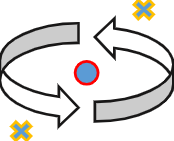
\includegraphics[width=0.3\textwidth]{eddy-shape.png}
    \caption{Query Pair of Points}
    \label{Fig_EddyShape} 
    \end{center}
  \end{figure}

  \newpage
  \item{test-eddy-std\\}

  Control: Automatic
            
  Initial State: Empty flow field, zero $\mathbf{u_{avg}}$
            
  Input:
  \begin{itemize}
    \item Profile: 1 eddy with predetermined orientation\\
    $\mathbf{x}=(0,0,0)$\tab$\sigma=1$\\
    $\alpha=(0,0,1)$ (intensity = 1, orientation along z-axis)
    \item Query: Mesh grid of points covering the eddy
  \end{itemize}
  Output: Velocity vectors at each point $\mathbf{u}$\\
  Expected behavior:
  \begin{itemize}
    \item $\text{std}(\mathbf{u_z}) < \text{tol}$
  \end{itemize}

  Test Case Derivation: Flow of an eddy should be around its orientation axis. Thus, velocity standard deviation along the eddy orientation should be zero (below tolerance).
            
  How test will be performed: Automated test script, GitHub Actions.

  \begin{figure}[h!]
    \begin{center}
    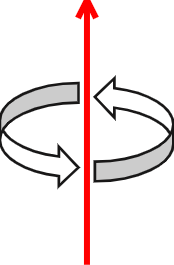
\includegraphics[width=0.3\textwidth]{eddy-orient.png}
    \caption{Eddy Orientation}
    \label{Fig_EddyOrient} 
    \end{center}
  \end{figure}

\end{enumerate}

\newpage
\subsubsection{Field Genration Test} \label{FieldGenTest}
\paragraph{Generation of Flow Field [R2]}

\begin{enumerate}

  \item{test-field-sum\\}

  Control: Automatic
            
  Initial State: Empty flow field, $\mathbf{u_{avg}}$
            
  Input:
  \begin{itemize}
    \item Profile: Any number of eddies, random orientations
    \item Query: Mesh grid of points of the entire flow field at any $t$
  \end{itemize}
  Output: Velocity vectors at each point: $\mathbf{u}$\\
  Expected behavior:
  \begin{itemize}
    \item $|\sum\mathbf{u}-\mathbf{u_{avg}}| < \text{tol}$
  \end{itemize}

  Test Case Derivation: The vector sum of all velocity fluctuations caused by the eddies should be zero (below tolerance).
            
  How test will be performed: Automated test script, GitHub Actions.

  \item{test-field-std-time\\}

  Control: Automatic
            
  Initial State: Empty flow field, $\mathbf{u_{avg}}$
            
  Input:
  \begin{itemize}
    \item Profile: Any number of eddies, random orientations
    \item Query: Mesh grid of points of the entire flow field\\
    $t_0=0$\tab$t_1=10$
  \end{itemize}
  Output: Velocity vectors at each point: $\mathbf{u}$\\
  Expected behavior:
  \begin{itemize}
    \item $\text{std}(\mathbf{u})|_{t_0} - \text{std}(\mathbf{u})|_{t_1} < \text{tol}$
  \end{itemize}

  Test Case Derivation: Velocity standard deviation should stay the same regardless of time.

  How test will be performed: Automated test script, GitHub Actions.

  \item{test-field-std-intensity\\}

  Control: Automatic
            
  Initial State: Empty flow field, $\mathbf{u_{avg}}$
            
  Input:
  \begin{itemize}
    \item Profile: Any number of eddies, random orientations\\
    Increasing eddy intensity $|\mathbf{\alpha}|$
    \item Query: Mesh grid of points of the entire flow field
  \end{itemize}
  Output: Velocity vectors at each point: $\mathbf{u}$\\
  Expected behavior:
  \begin{itemize}
    \item if $|\mathbf{\alpha}|_1 > |\mathbf{\alpha}|_2$ then $\text{std}(\mathbf{u})_1 > \text{std}(\mathbf{u})_2$
  \end{itemize}

  Test Case Derivation: Velocity standard deviation should increase with eddy intensity $|\mathbf{\alpha}|$.

  How test will be performed: Automated test script, GitHub Actions.

\end{enumerate}

\subsubsection{Divergence Test} \label{DivergenceFree}
\paragraph{Divergence Free Condition [R4]} 

\begin{enumerate}

  \item{test-field-divergence\\}

  Control: Automatic
            
  Initial State: Empty flow field, $\mathbf{u_{avg}}$
            
  Input:
  \begin{itemize}
    \item Profile: Any number of eddies, random orientations
    \item Query: Mesh grid of points of the entire flow field
  \end{itemize}
  Output: Velocity vectors at each point: $\mathbf{u}$\\
  Expected behavior:
  \begin{itemize}
    \item $\text{div}(\mathbf{u}) < \text{tol}$
  \end{itemize}

  Test Case Derivation: The flow field should be divergence-free.

  How test will be performed: Automated test script, GitHub Actions.

\end{enumerate}

\subsubsection{Eddy Profile} \label{EddyProfile}
\paragraph{Provide Realistic Profile Before Generation [R3]\\}
Test case for this requirement will be added in the future given more theoretical background.

\subsubsection{CFD Interface} \label{CFDInterface}
\paragraph{Feed IC and BC to CFD Software [R5]\\}

\begin{enumerate}

  \item{test-cfd-interface\\}
  
  Type: Manual.
            
  Initial State: Empty flow field, $\mathbf{u_{avg}}$
            
  Input:
  \begin{itemize}
    \item Profile: Any number of eddies, random orientations
    \item Query: CFD software should query points in the flow field
  \end{itemize}
  Output: Velocity vectors at each point: $\mathbf{u}$\\
  Expected behavior:
  \begin{itemize}
    \item They should be feed into the CFD software
  \end{itemize}

  Test Case Derivation: The CFD software should be able get the flow field generated by \progname{} as IC and BC.

  How test will be performed: Manually perform a CFD simulation in conjecture with  \progname{}.
\end{enumerate}

\newpage
\subsection{Tests for Nonfunctional Requirements} \label{NonfuncTest}
NFR1, NFR2 and NFR4 is already covered by functional test of CFD interface (\ref{CFDInterface}). NFR3 (maintainability) will be verified by a separate test detailed below.
% \wss{The nonfunctional requirements for accuracy will likely just reference the
%   appropriate functional tests from above.  The test cases should mention
%   reporting the relative error for these tests.  Not all projects will
%   necessarily have nonfunctional requirements related to accuracy}

% \wss{Tests related to usability could include conducting a usability test and
%   survey.  The survey will be in the Appendix.}

% \wss{Static tests, review, inspections, and walkthroughs, will not follow the
% format for the tests given below.}

\subsubsection{Maintainability} \label{MaintTest}
		
\paragraph{Modifying Shape Function\\}
In terms of maintainability, users who looks to modify \progname{} would most likely want to change the shape functions of the eddies to fit their specific needs. If the software is well structured and documented, they should be able to do so with ease, even without systematic programming knowledge.

\begin{enumerate}

\item{test-modify-shape-func\\}

Type: Static
					
Initial State: Reviewer is provided with documentation and source code, and no other help.
					
Input/Condition: Reviewer is given a mathematical equation for a new shape function.
					
Output/Result: Reviewer should be able to modify the source code to implement the new shape function.
					
How test will be performed: Performed by volunteers or potential users of the software. Time taken will be recorded. Check if the modified software still passes the automated functional tests.

\end{enumerate}

\newpage
\subsection{Traceability Between Test Cases and Requirements}
\begin{table}[h!]
  \centering
  \begin{tabular}{|c|c|c|c|c|c|c|c|c|c|c|c|c|c|c|c|c|c|c|c|}
  \hline
                            & R1 & R2 & R3 & R4 & R5 & NFR1 & NFR2 & NFR3 & NFR4 \\
  \hline
  Test \ref{InputTest}      & X  &    &    &    &    &      &      &      &      \\\hline
  Test \ref{EddyGenTest}    &    & X  &    &    &    &      &      &      &      \\\hline
  Test \ref{FieldGenTest}   &    & X  &    &    &    &      &      &      &      \\\hline
  Test \ref{DivergenceFree} &    &    &    & X  &    &      &      &      &      \\\hline
  Test \ref{EddyProfile}    &    &    & X  &    &    &      &      &      &      \\\hline
  Test \ref{CFDInterface}   &    &    &    &    & X  & X    & X    &      & X    \\\hline
  Test \ref{MaintTest}      &    &    &    &    &    &      &      & X    &      \\\hline
  \end{tabular}
  \caption{Traceability Between Test Cases and Requirements}
  \label{Table:A_trace}
\end{table}

% \wss{Provide a table that shows which test cases are supporting which
%   requirements.}

\section{Unit Test Description}

\wss{This section should not be filled in until after the MIS (detailed design
  document) has been completed.}

\wss{Reference your MIS (detailed design document) and explain your overall
philosophy for test case selection.}  

\wss{To save space and time, it may be an option to provide less detail in this section.  
For the unit tests you can potentially layout your testing strategy here.  That is, you 
can explain how tests will be selected for each module.  For instance, your test building 
approach could be test cases for each access program, including one test for normal behaviour 
and as many tests as needed for edge cases.  Rather than create the details of the input 
and output here, you could point to the unit testing code.  For this to work, you code 
needs to be well-documented, with meaningful names for all of the tests.}

\subsection{Unit Testing Scope}

\wss{What modules are outside of the scope.  If there are modules that are
  developed by someone else, then you would say here if you aren't planning on
  verifying them.  There may also be modules that are part of your software, but
  have a lower priority for verification than others.  If this is the case,
  explain your rationale for the ranking of module importance.}

\subsection{Tests for Functional Requirements}

\wss{Most of the verification will be through automated unit testing.  If
  appropriate specific modules can be verified by a non-testing based
  technique.  That can also be documented in this section.}

\subsubsection{Module 1}

\wss{Include a blurb here to explain why the subsections below cover the module.
  References to the MIS would be good.  You will want tests from a black box
  perspective and from a white box perspective.  Explain to the reader how the
  tests were selected.}

\begin{enumerate}

\item{test-id1\\}

Type: \wss{Functional, Dynamic, Manual, Automatic, Static etc. Most will
  be automatic}
					
Initial State: 
					
Input: 
					
Output: \wss{The expected result for the given inputs}

Test Case Derivation: \wss{Justify the expected value given in the Output field}

How test will be performed: 
					
\item{test-id2\\}

Type: \wss{Functional, Dynamic, Manual, Automatic, Static etc. Most will
  be automatic}
					
Initial State: 
					
Input: 
					
Output: \wss{The expected result for the given inputs}

Test Case Derivation: \wss{Justify the expected value given in the Output field}

How test will be performed: 

\item{...\\}
    
\end{enumerate}

\subsubsection{Module 2}

...

\subsection{Tests for Nonfunctional Requirements}

\wss{If there is a module that needs to be independently assessed for
  performance, those test cases can go here.  In some projects, planning for
  nonfunctional tests of units will not be that relevant.}

\wss{These tests may involve collecting performance data from previously
  mentioned functional tests.}

\subsubsection{Module ?}
		
\begin{enumerate}

\item{test-id1\\}

Type: \wss{Functional, Dynamic, Manual, Automatic, Static etc. Most will
  be automatic}
					
Initial State: 
					
Input/Condition: 
					
Output/Result: 
					
How test will be performed: 
					
\item{test-id2\\}

Type: Functional, Dynamic, Manual, Static etc.
					
Initial State: 
					
Input: 
					
Output: 
					
How test will be performed: 

\end{enumerate}

\subsubsection{Module ?}

...

\subsection{Traceability Between Test Cases and Modules}

\wss{Provide evidence that all of the modules have been considered.}
				
\bibliographystyle{plainnat}

\bibliography{../../refs/References}

\newpage

\section{Appendix}

% This is where you can place additional information.

\subsection{Symbolic Parameters} \label{secSymParams}

The definition of the test cases will call for SYMBOLIC\_CONSTANTS.
Their values are defined in this section for easy maintenance.

\begin{itemize}
  \item Tolerance: some small value, e.g. $\text{tol}=0.0001$
  \item Average velocity: along x-axis (1D flow), e.g. $\mathbf{u_{avg}}=(5,0,0)$
\end{itemize}


% \subsection{Usability Survey Questions?}

% \wss{This is a section that would be appropriate for some projects.}

% \newpage{}
% \section*{Appendix --- Reflection}

% The information in this section will be used to evaluate the team members on the
% graduate attribute of Lifelong Learning.  Please answer the following questions:

% \newpage{}
% \section*{Appendix --- Reflection}

% \wss{This section is not required for CAS 741}

% The information in this section will be used to evaluate the team members on the
% graduate attribute of Lifelong Learning.  Please answer the following questions:

% \begin{enumerate}
%   \item What knowledge and skills will the team collectively need to acquire to
%   successfully complete the verification and validation of your project?
%   Examples of possible knowledge and skills include dynamic testing knowledge,
%   static testing knowledge, specific tool usage etc.  You should look to
%   identify at least one item for each team member.
%   \item For each of the knowledge areas and skills identified in the previous
%   question, what are at least two approaches to acquiring the knowledge or
%   mastering the skill?  Of the identified approaches, which will each team
%   member pursue, and why did they make this choice?
% \end{enumerate}

\end{document}